\documentclass{standalone}
\usepackage{tikz}
\begin{document}
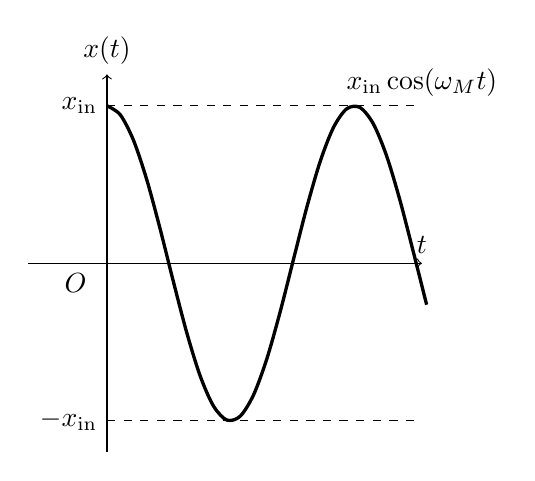
\begin{tikzpicture}[scale=2]
    \node[below] at (-3.2,0) {$O$};
    \draw[->] (-3.5, 0) -- (-1, 0) node[above]{$t$};
    \draw[->] (-3,-1.2)--(-3,1.2)node[above]{$x(t)$};
    \draw[very thick] plot[smooth, domain=-3:-0.97] (\x, {cos(4*(\x+3) r)});
    \draw[dashed] (-3,1) node[left] {$x_\mathrm{in}$} -- (-1,1) node[above]{$x_\mathrm{in}\cos(\omega_M t)$};
    \draw[dashed] (-3,-1) node[left] {$-x_\mathrm{in}$} -- (-1,-1);
\end{tikzpicture}
\end{document}